\section{Darboux Property for Derivatives}

\begin{theorem}[Darboux property]
  \label{th:darboux}%
    Let $f\colon I \to \RR$ be a differentiable function on an interval
  $I\subset \RR$.
  Then the derivative satisfies the intermediate value property:
  if $a,b\in I$, $a\neq b$, then for every $m\in \openinterval{f'(a)}{f'(b)}$ 
  \mynote{It is understood that $\openinterval{f'(a)}{f'(b)} = \openinterval{f'(b)}{f'(a)}$ 
  if $f'(b)<f'(a)$.}%
  (that is, $m$ is an intermediate value between 
  $f'(a)$ and $f'(b)$)
  there exists $x\in(a,b)$ such that $f'(x) = m$. 
\end{theorem}
\begin{proof}
Given $x,y\in [a,b]$, $x\neq y$, we can consider 
the difference quotient:
  \[
    R(x,y) = \frac{f(y)-f(x)}{y-x}.
  \]
Fixing $x=a$, the function $y\mapsto R(a,y)$ is continuous and tends to $f'(a)$
as $y$ approaches $a$.
Thus, by the intermediate value theorem~\ref{th:valori_intermedi},
this function takes all values between $f'(a)$ and 
$R(a,b)$. Similarly, fixing $y=b$, the function $x\mapsto R(x,b)$ 
is continuous and tends to $f'(b)$ as $x$ approaches $b$.
Thus, this function takes all intermediate values 
between $R(a,b)$ and $f'(b)$. 
Therefore, there exist $x,y$ such 
that $R(x,y)=m$ and, by Lagrange's theorem~\ref{th:lagrange},
there will exist an intermediate point $t\in(x,y)$ where 
$f'(t)=R(x,y) = m$.
\end{proof}

\newsavebox{\qrdarboux}\sbox{\qrdarboux}{\myurlhere{darboux}{Function with non-continuous derivative example \getrefnumber{ex:derivata_non_continua}}}%
\begin{figure}
  \centering
\includegraphics[height=4cm]{darboux.pdf}
  \centering
\includegraphics[width=\textwidth]{darboux2.pdf}
  \begin{comment}
  \begin{tikzpicture}[scale=5]
    \draw[->] (-0.5, 0) -- (0.5, 0) node[above] {$x$};
    \draw[->] (0, -0.3) -- (0, 0.3) node[right] {$y$};
    \draw[domain=-0.51:0.5, smooth, variable=\x, gray] plot ({\x}, {\x*\x});
    \draw[domain=-0.51:0.5, smooth, variable=\x, gray] plot ({\x}, {-\x*\x});
    \draw[domain=-0.51:0.5, variable=\x, samples=200, blue, thick] plot ({\x}, {\x*\x*sin(deg(1/\x))});
  \end{tikzpicture}
  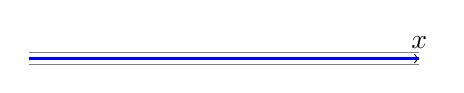
\begin{tikzpicture}[scale=5000]
    \draw[->] (0.0045, 0) -- (0.0055, 0) node[above] {$x$};
    \draw[domain=0.0045:0.0055, smooth, variable=\x, gray] plot ({\x}, {\x*\x});
    \draw[domain=0.0045:0.0055, smooth, variable=\x, gray] plot ({\x}, {-\x*\x});
    \draw[domain=0.0045:0.0055, variable=\x, samples=200, blue, thick] plot ({\x}, {\x*\x*sin(deg(1/\x))});
  \end{tikzpicture}
  \end{comment}
  \caption{The graph of a differentiable function with 
    a non-continuous derivative (see example~\ref{ex:derivata_non_continua}).
    The magnification in the lower drawing makes it evident 
    that the derivative oscillates between the values 
    $-1$ and $1$ in every neighborhood of $0$.
    The Darboux property (theorem~\ref{th:darboux})
    is still satisfied: the derivative takes all values 
    between $1$ and $-1$ in every neighborhood of $x=0$ but 
    does not have a limit as $x\to 0$.\\\\
    \usebox{\qrdarboux}
}
\end{figure}

\begin{example}
[differentiable function with non-continuous derivative]
\label{ex:derivata_non_continua}%
\mymark{**}%
\index{function!differentiable with non-continuous derivative}%
\index{derivative!non-continuous}%
The function $f\colon \RR \to \RR$ defined by
\[
  f(x)
  = \begin{cases}
    x^2 \sin(1/x) & \text{if $x \neq 0$} \\
    0 & \text{if $x=0$.}
  \end{cases}
\]
is differentiable on all of $\RR$, $f'(0)=0$, but the limit
\[
\lim_{x\to 0} f'(x)
\]
does not exist (and thus $f'\colon \RR\to\RR$ is not continuous at $x=0$).
\end{example}
%
\begin{proof}
The function $x^2 \sin(1/x)$ is infinitely differentiable on its entire domain
$\RR\setminus\ENCLOSE{0}$ as it is a composition of elementary functions that
are infinitely differentiable.
Thus, by the locality of the derivative, the function $f$ is also infinitely
differentiable on $\RR\setminus\ENCLOSE{0}$.
For $x\neq 0$, we can then compute $f'(x)$ using the differentiation rules
\[
  f'(x)
  = D \enclose{x^2\sin \frac 1 x}
  = 2x \sin \frac 1 x + x^2 \enclose{\cos \frac 1 x} \cdot\frac{-1}{x^2}
  = 2x \sin \frac 1 x - \cos \frac 1 x.
\]

We now verify that $f$ is continuous and differentiable at $0$.
Indeed, we have
\[
 \lim_{h\to 0}\frac{f(0+h)-f(0)}{h}
 = \lim_{h\to 0} h \sin \frac 1 h = 0
\]
and thus $f'(0) = 0$.
However, observe that $f'(x)$ does not have a limit as $x\to 0$
since for $x \to 0$, $2x \sin(1/x) \to 0$, but the limit of $\cos (1/x)$ does
not exist. Thus, $f'(x)$ is the sum of a function that has a zero limit and a
function whose limit does not exist as $x\to 0$. Therefore, $f'(x)$ does not
have a limit as $x\to 0$.
\end{proof}

\begin{proposition}[differentiability criterion]%
\label{prop:4384774}\mymark{**}%
Let $I\subset \RR$ be an interval, $x_0\in I$,
$f\colon I \to \RR$ a function continuous on all of $I$ 
and differentiable in $I\setminus\ENCLOSE{x_0}$.
If the limit of the derivative
\[
  \lim_{x\to x_0} f'(x) = m
\]
exists and is finite, then the function $f$ is differentiable at $x_0$ and
$f'(x_0) = m$.
\end{proposition}
%
\begin{proof}
\mymark{*}
Consider a generic point $x>x_0$ (the case $x<x_0$ is entirely analogous).
By Lagrange's theorem, we know there exists a point $y\in (x_0,x)$ such that
\[
  \frac{f(x)-f(x_0)}{x-x_0} = f'(y).
\]
As $x\to x_0$, it follows that $y\to x_0$, and thus
the limit of the difference quotient exists:
\[
  f'(x_0) = \lim_{x\to x_0} \frac{f(x)-f(x_0)}{x-x_0}
  = \lim_{y\to x_0} f'(y) = m.
\]
\end{proof}
%
The previous proposition states that the derivative of a function at a
point cannot have a value different from its limit, if such a limit exists.
However, there exist differentiable functions whose derivative is not
continuous, as we have seen
in example~\ref{ex:derivata_non_continua}
since the limit of the derivative might not exist.